\section{Correctness}
\label{sec:correctness}

To evaluate Brel's correctness, we will use Charles Hoffman's XBRL conformance suite \cite{hoffman_conformance_suite}.
The conformance suite contains a set of XBRL reports that are known to be correct.
It checks for conformance to the XBRL specification from both a syntactic and a logical point of view.
Brel will ignore the logical checks, as it only deals with the syntactic part of the XBRL specification.

We will not cover either the SEC's or the ESMA's conformance suites, 
as they contain many test cases that are not relevant to Brel in its current state.

Besides the conformance suite, we will also look at a hand-picked XBRL report.
Since the source files of an XBRL report are not human-readable, 
we will use the XBRL platform Arelle\cite{arelle} to visualize the structures that Brel extracts from the reports.
% We will compare the structures that Brel extracts from them against the structures that the XBRL specification prescribes.
Arelle closely follows the XBRL specification and can therefore be considered a reliable source of truth.
We will compare the structures that Brel extracts from the reports against the structures that Arelle extracts from the same reports.
For the sake of brevity, we will only look at a single network within the report.
Even though this evaluation only covers a single component within the report,
it will give us a more intuitive understanding of Brel's correctness compared to the conformance suite.
Brel also contains its own test suite, which is not covered in this thesis.

\subsection{Conformance suite}

Charles Hoffman maintains a conformance suite for XBRL \cite{hoffman_conformance_suite}.
It covers both the syntactic and the semantic aspects of the XBRL specification.
The conformance suite contains a set of XBRL reports that are known to be correct or incorrect.
It checks for conformance to the XBRL specification from both a syntactic and a logical point of view.

Since Brel only deals with the syntactic part of the XBRL specification, 
it will be unable to check the logical part of the conformance suite.
Therefore reports that are syntactically correct, but semantically incorrect, will be considered correct by Brel.

Figure \ref{fig:conformance_suite} shows the results of running the conformance suite on Brel.

\begin{figure}[H]
  \centering
  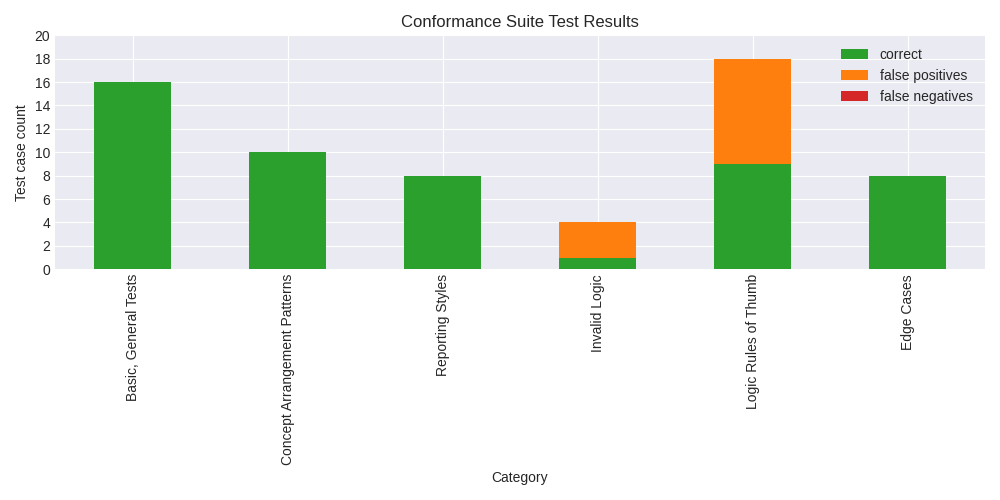
\includegraphics[width=1\textwidth]{images/seattle_method_test_results.png}
    \caption{Conformance suite results}
    \label{fig:conformance_suite}
\end{figure}

The conformance suite contains 77 test cases, of which 22 are considered logical checks.
Of the 22 logical checks, Brel passes 10 and fails 12.
Since Brel only deals with the syntactic part of the XBRL specification,
the test cases it passed it passed by coincidence.
We still list the results for completeness.

Of the 55 syntactic checks, Brel passes all of them.
This is a good result, as it shows that Brel is able to parse XBRL reports correctly.
However, it is important to note that the conformance suite is not exhaustive.
Also, conformance suite test cases are not necessarily representative of real-world XBRL reports.
They serve as a good starting point, but they are not enough to guarantee Brel's correctness.

\subsection{Hand-picked XBRL reports}

We will also look at a hand-picked XBRL report.
We will compare the structures that Brel extracts from them against the structures that the XBRL specification prescribes.
Since the source files of an XBRL report meant to be read by machines,
we will use the XBRL platform Arelle to visualize the structures that Brel extracts from the reports.
Arelle is a mature, robust and widely used XBRL platform and can therefore be considered a reliable source of truth.
It closely follows the XBRL specification, including the OIM.

% The hand-picked XBRL reports are:

% A report from the SEC's EDGAR database \cite{sec_edgar}. 
The hand picked report is from the SEC's EDGAR database \cite{sec_edgar}.
In this case we will use Microsoft's 10K report for the fiscal year 2022.
\footnote{Available at \url{https://www.sec.gov/ixviewer/ix.html?doc=/Archives/edgar/data/789019/000095017023035122/msft-20230630.htm}}
This report will be loaded directly from the EDGAR database by providing the URL of the report to Brel.
% A report from the ESMA's ESEF database hosted by the XBRL Foundation\cite{esma_database}.
% In this case we will use Novo Nordisk's 2023 financial report covering the first three quarters of 2023.
% \footnote{Available at \url{https://filings.xbrl.org/filing/549300DAQ1CVT6CXN342-2023-09-30-ESEF-DK-0}}
% This report will be loaded from disk.

% We will look at the \texttt{DocumentAndEntityInformation} component and all facts associated with the concepts within its presentation network.
% It acts as a cover page for the report and contains information about the company, the report, and the auditor.
% Its presentation network is a good starting point, since the information in it is understandable by non-accountants.
% Furthermore, Brel employs the same network parsing algorithm for all networks, so the results of this evaluation will be representative of Brel's correctness.
We will look at the \texttt{ComprehenisveIncomeStatement} component and all facts associated with the concepts within its presentation network.
Its presentation network acts as a good sanity check, since the information in it is understandable by non-accountants.
Furthermore, Brel employs the same network parsing algorithm for all networks, so the results of this evaluation will be representative of Brel's correctness.

% The following sections show the results of the evaluation.
% The report is loaded directly from the EDGAR database by providing the URL of the report to Brel.
% First, let us look at the cover page as it is presented in Arelle.
First, let us look at the comprehensive income statement as it is presented in Arelle.

\begin{figure}[H]
  \centering
%   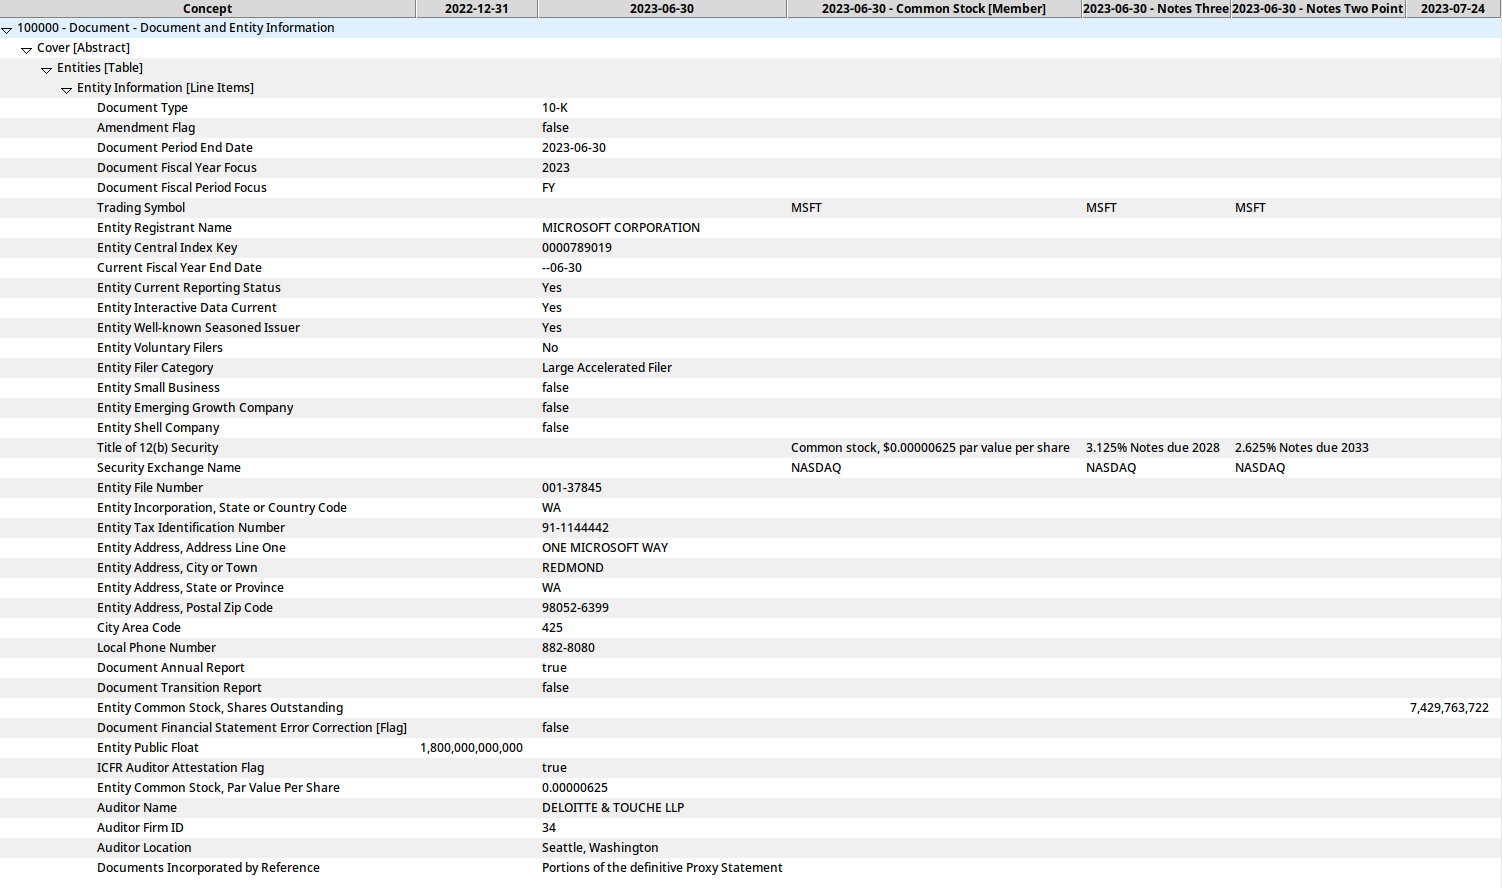
\includegraphics[width=1\textwidth]{images/msft_coverpage_arelle.png}
    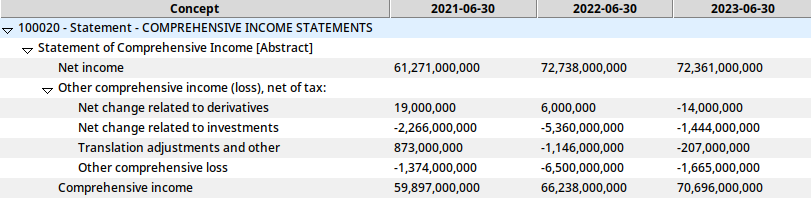
\includegraphics[width=1\textwidth]{images/msft_income_statement_arelle.png}
    \caption{Microsoft's 10K report cover page in Arelle}
    \label{fig:msft_income_statement_arelle}
\end{figure}

% The figure \ref{fig:msft_coverpage_arelle} shows the cover page of Microsoft's 10K report in Arelle.
The figure \ref{fig:msft_income_statement_arelle} shows the comprehensive income statement of Microsoft's 10K report in Arelle.
Brel works different from Arelle, as it does not visualize the network and its facts in a graphical manner.
However, using the \texttt{viewer.py} script we have written in section \ref{sec:usability}, 
we can visualize the cover page in a textual manner.
The figure \ref{fig:msft_income_statement_network} shows the hierarchy of cover page of Microsoft's 10K report in Brel.

\begin{figure}[H]
    \begin{lstlisting}[basicstyle=\small\ttfamily]
Component: .../Role_StatementCOMPREHENSIVEINCOMESTATEMENTS
Info: 100020 - Statement - COMPREHENSIVE INCOME STATEMENTS

link name: link:presentationLink
arc roles: ['.../parent-child'], arc name: link:presentationArc
└──[ABSTRACT] Statement of Comprehensive Income [Abstract]
    ├──[CONCEPT] Net Income (Loss)
    ├──[ABSTRACT] Other comprehensive income (loss), net of tax:
    │  ├──[CONCEPT] Net change related to derivatives
    │  ├──[CONCEPT] Net change related to investments
    │  ├──[CONCEPT] Translation adjustments and other
    │  └──[CONCEPT] Other comprehensive income (loss)
    └──[CONCEPT] Comprehensive Income (Loss), Net of Tax, Attributable to Parent
    \end{lstlisting}
    \caption{Microsoft's 10K presentation network in Brel}
    \label{fig:msft_income_statement_network}
\end{figure}

The figure \ref{fig:msft_income_statement_network} shows the hierarchy of the comprehensive income statement of Microsoft's 10K report in Brel.
Note that the labels between the two figures are different, since Arelle might use different label roles from the ones used in Brel.
The only difference between the content of the two figures is the fact that Arelle includes the facts associated with the concepts in the network, 
while Brel only includes the report elements and their relationships.

Luckily, we can use the \texttt{viewer.py} and filter all facts that have concepts present in figure \ref{fig:msft_income_statement_network}
to visualize the facts associated with the concepts in the network.
The output of the \texttt{viewer.py} script is shown in figure \ref{fig:msft_income_statement_facts}.
Note that the output has been truncated.
Also note that XBRL reports can contain duplicate facts, as they can be reported in different contexts.
Arelle does not show duplicate facts, while Brel does.

\begin{figure}[H]
  \begin{lstlisting}[basicstyle=\tiny\ttfamily]
+-------------------------------------------------------------------------------------------------------------------------+
| Facts Table                                                                                                             |
+------------------------------------------------------+-------------------------------+------------+-------+-------------+
|                                              concept |                        period |     entity |  unit |       value |
+------------------------------------------------------+-------------------------------+------------+-------+-------------+
|                                us-gaap:NetIncomeLoss | from 2020-07-01 to 2021-06-30 | 0000789019 |  USD  | 61271000000 |
|                                us-gaap:NetIncomeLoss | from 2021-07-01 to 2022-06-30 | 0000789019 |  USD  | 72738000000 |
|                                us-gaap:NetIncomeLoss | from 2022-07-01 to 2023-06-30 | 0000789019 |  USD  | 72361000000 |
|           us-gaap:OtherComprehensiveIncomeLossCas... | from 2020-07-01 to 2021-06-30 | 0000789019 |  USD  |    19000000 |
|           us-gaap:OtherComprehensiveIncomeLossCas... | from 2021-07-01 to 2022-06-30 | 0000789019 |  USD  |     6000000 |
|           us-gaap:OtherComprehensiveIncomeLossCas... | from 2022-07-01 to 2023-06-30 | 0000789019 |  USD  |   -14000000 |
|               us-gaap:OtherComprehensiveIncomeLos... | from 2020-07-01 to 2021-06-30 | 0000789019 |  USD  | -2266000000 |
|               us-gaap:OtherComprehensiveIncomeLos... | from 2021-07-01 to 2022-06-30 | 0000789019 |  USD  | -5360000000 |
|               us-gaap:OtherComprehensiveIncomeLos... | from 2022-07-01 to 2023-06-30 | 0000789019 |  USD  | -1444000000 |
| us-gaap:OtherComprehensiveIncomeLossForeignCurren... | from 2020-07-01 to 2021-06-30 | 0000789019 |  USD  |   873000000 |
| us-gaap:OtherComprehensiveIncomeLossForeignCurren... | from 2021-07-01 to 2022-06-30 | 0000789019 |  USD  | -1146000000 |
| us-gaap:OtherComprehensiveIncomeLossForeignCurren... | from 2022-07-01 to 2023-06-30 | 0000789019 |  USD  |  -207000000 |
|                        us-gaap:OtherComprehensive... | from 2020-07-01 to 2021-06-30 | 0000789019 |  USD  | -1374000000 |
|                        us-gaap:OtherComprehensive... | from 2021-07-01 to 2022-06-30 | 0000789019 |  USD  | -6500000000 |
|                        us-gaap:OtherComprehensive... | from 2022-07-01 to 2023-06-30 | 0000789019 |  USD  | -1665000000 |
|                  us-gaap:ComprehensiveIncomeNetOfTax | from 2020-07-01 to 2021-06-30 | 0000789019 |  USD  | 59897000000 |
|                  us-gaap:ComprehensiveIncomeNetOfTax | from 2021-07-01 to 2022-06-30 | 0000789019 |  USD  | 66238000000 |
|                  us-gaap:ComprehensiveIncomeNetOfTax | from 2022-07-01 to 2023-06-30 | 0000789019 |  USD  | 70696000000 |
+------------------------------------------------------+-------------------------------+------------+-------+-------------+
    \end{lstlisting}
    \caption{Microsoft's 10K facts in Brel}
    \label{fig:msft_income_statement_facts}
\end{figure}

The figure \ref{fig:msft_income_statement_facts} clearly shows that Brel is able to extract the facts from the comprehensive income statement of Microsoft's 10K report correctly.
All facts present in figure \ref{fig:msft_income_statement_arelle} are also present in figure \ref{fig:msft_income_statement_facts} and vice versa.
Each individual fact is also correct, as it is associated with the correct concept, period, entity, unit, and value.
Brel represents these characteristics differently from Arelle.
For example, Arelle visualizes concepts using their labels, while Brel visualizes concepts using their QNames.
However, the values themselves represent the same information.
The only difference is between the representation of the facts, as Arelle visualizes the facts as a table, where the rows are the concepts and the columns are the periods.
Brel visualizes the facts as a table representing a hypercube.

We can conclude that Brel is able to extract the structures from the comprehensive income statement of Microsoft's 10K report correctly.
This is a good result, as it shows that Brel is able to parse XBRL reports correctly.
However, it is important to note that this evaluation only covers a single component within the report.
It does not cover the full range of Brel's functionality or its correctness.
This example serves as a vertical slice of Brel's correctness.
Together with the conformance suite, it gives us a good idea of Brel's correctness.
